\documentclass[twoside,11pt]{article}

\usepackage{jmlr2e}

% Heading arguments are {volume}{year}{pages}{submitted}{published}{author-full-names}
\jmlrheading{7}{2016}{1-5}{7/16}{-}{Guillaume Lema\^itre, Fernando Nogueira, and Dayvid V. R. Oliveira}

% Short headings should be running head and authors last names
\ShortHeadings{A python toolbox to tackle the curse of imbalanced datasets in machine learning}{Lema\^itre, Nogueira, and Victor}
\firstpageno{1}

\begin{document}

\title{A python toolbox to tackle the curse of imbalanced datasets in machine learning}
\author{Guillaume Lema\^itre \email g.lemaitre58@gmail.com \\ 
    \addr{LE2I UMR6306, CNRS, Arts et M\'etiers, Universit\'e Bourgogne Franche-Comt\'e} \\ 
    \addr{12 rue de la Fonderie, 71200 Le Creusot, France} \\ 
    \addr{ViCOROB, Universitat de Girona} \\ 
    \addr{Campus Montilivi, Edifici P4, 17071 Girona, Spain}
        \AND
        Fernando Nogueira \email fmfnogueira@gmail.com \\ 
        \addr{theScore, Inc.} \\ 
        \addr{500 King Street West 4\textsuperscript{th} Floor Toronto, Ontario M5V1L9 Canada}
        \AND
        Dayvid V. R. Oliveira \email dvro@cin.ufpe.br \\ 
        \addr{VIISAR Research Group, Centro de Inform\'atica - Universidade Federal de Pernambuco} \\ 
        %\addr{Av. Prof. Luiz Freire, s/n - Cidade Universitária Recife - PE, 50740-540, Brazil}} 
        \addr{Av. Jornalista Aníbal Fernandes, s/n - Cidade Universitária - PE, 50740-560, Brazil}} 
\editor{-}

\maketitle

\begin{abstract}
\emph{UnbalancedDataset} is an open-source python toolbox aiming at providing a wide range of methods to cope with the problem of imbalanced dataset frequently encountered in machine learning and pattern recognition.
The state-of-the-art methods implemented can be categorized into 4 different sampling strategies: (i) under-sampling, (ii) over-sampling, (iii) combination of over- and under-sampling, and (iv) ensemble learning methods.
The proposed toolbox only depends of \emph{numpy}, \emph{scipy}, and \emph{scikit-learn} and is distributed under MIT license.
The implementation pattern is identical to the \emph{scikit-learn} API to offer compatibility.
Documentation, unit tests as well as integration tests are provided to allow new developers to contribute.
The toolbox is publicly available in GitHub \url{https://github.com/fmfn/UnbalancedDataset} as well as the documentation \url{https://github.io}.
\end{abstract}

\begin{keywords}
Imbalanced Dataset, Over-Sampling, Under-Sampling, Ensemble Learning, Machine Learning, Python.
\end{keywords}

\section{Introduction}

Many real world datasets have many samples of some classes (majority classes),
and only a few samples the other class (minority classes). This imbalance gives
rise to the ``class imbalance'' problem~\cite{prati2009data} (or ``curse of imbalanced datasets'')
which is the problem of learning a concept from the class that has a small number of samples compared
to the other classes. 

The class imbalance problem has been encountered in multiple areas such as 
telecommunication managements, bioinformatics, fraud detection, and medical diagnosis,
and has been considered one of the top 10 problems in data mining and 
pattern recognition~\cite{10problemsInDM:2006}. 
Medical data, for example, are prone to suffer from class imbalance due to the fact 
that the portion of diseased patients is far lower than healthy patients,
and the detection and classification of minority diseased patients are highly essential
so that they can be treated as soon as possible.

Imbalanced data substantially compromises the learning process, since most of the 
standard machine learning algorithms expect balanced class distribution or an 
equal misclassification cost~\cite{he2009learning}. For this reason, several
approaches have been specifically proposed to handle such datasets.

In this paper, we present the \textbf{UnbalancedDataset} API, 
\textit{a python toolbox to tackle the curse of imbalanced datasets
in machine learning}. The following sections present the implemented
methods, implemented design, sustainability and continuous integration details,
and finally, the conclusion of this paper, including future functionalities
for the UnbalancedDataset API.

%This problem is frequently referred as ``class imbalance'' problem~\cite{prati2009data} and has been encountered in multiple areas such as telecommunication managements, bioinformatics, fraud detection, and medical diagnosis. 
%Imbalanced data substantially compromises the learning process since most of the standard machine learning algorithms expect balanced class distribution or an equal mis-classification cost~\cite{he2009learning}.
%Medical data are prone to such drawbacks due to the fact that the portion of diseased samples or patients is far lower than healthy cases.
%Furthermore, the detection and classification of minority malignant cases are highly essential so that the sensitivity of developed algorithms need to be maximized.
%Consequently, the problem of imbalanced data is usually addressed by employing different techniques which do not impair the topology of the data.

\section{Project management}

\begin{description}
  \item[Quality insurance] In order to ensure code quality, a set of unit tests is provided leading to a coverage of 99 \% for the release 0.1 of the toolbox. Furthermore, the code quality is ensured by following \texttt{PEP8} standard and each contribution is automatically check through landscape.
  \item[Continuous integration]
  \item[Documentation]
\end{description}

In order to be sustainable and improved over years, the current toolbox offer a detailed documentation as well as a unit and integration tests.
A set of \emph{getting started} guide, examples, and API documentation is available.
The API documentation is automatically generated using \emph{sphinx} and \emph{numpydoc}.
A set of unit tests are implemented to allow back compatibility and integration of new pull-requests.
Furthermore, automatic continuous integration is also available through Travis CI.
Bugs can be reported through the issue tracker system provided by GitHub.

\section{Implementation design}

The implementation rely on \emph{numpy}, \emph{scipy}, and \emph{scikit-learn}.
The implementation pattern is identical to the \emph{scikit-learn} API to offer compatibility.
Each class implements 3 main functions inspired from the \emph{scikit-learn} API:
(i) \emph{fit} computes the parameter values which are later needed to transform the data into a balanced set;
(ii) \emph{transform} performs the sampling and return the data with the desired balancing ratio;
and (iii) \emph{fit\_transform} is equivalent of calling the function \emph{fit} follow the function \emph{transform}.

\section{Implemented methods}

Three strategies can be employed to overcome the problem of imbalanced datasets: 
(i) under-sampling, (ii) over-sampling, (iii) a combination of both, and (iv) ensemble learning.
The following sections give an overview of the techniques used to tackle this issue.

\subsection{Under-sampling}

Considering the problem of imbalanced, under-sampling is performed such that the number of samples of the majority class is reduced to be equal to the number of samples of the minority class.
The following methods are considered to perform such balancing.

\begin{description}
  \item[Random under-sampling] is performed by randomly selecting without replacement a subset of samples from the majority class such that the number of samples is then equal in both minority and majority classes.
  \item[Tomek links] can be used to under-sample the majority class of the original dataset~\cite{tomek1976two}.
Let define a pair of nearest neighbour samples $(x_i, x_j)$ such that their associated class label $y_i \neq y_j$.
The pair $(x_i, x_j)$ is defined as a Tomek link if, by relaxing the class label differentiation constraint, there is no other sample $x_k$ defined as the nearest neighbour of either $x_i$ or $x_j$.
Under-sampling is performed by removing the samples belonging to the majority class and forming a Tomek link.
It can be noted that this under-sampling strategy does not enforce a strict balancing between the majority and the minority classes.
  \item[Cluster centroids method] refers to the use of a $k$-means to cluster the feature space such that $k$ is set to be equal to the number of samples composing the minority class.
Hence, the centroids of these clusters define the new samples of the majority class. 
  \item[NearMiss] offers three different methods to under-sample the majority class~\cite{mani2003knn}.
In NearMiss-1, samples from the majority class are selected such that for each sample, the average distance to the $k$ nearest neighbour samples from the minority class is minimum.
NearMiss-2 diverges from NearMiss-1 by considering the $k$ farthest neighbours samples from the minority class.
In NearMiss-3, a subset $M$ containing samples from the majority class is generated by finding the $m$ nearest neighbours from each sample of the minority class.
Then, samples from the subset $M$ are selected such that for each sample, the average distance to the $k$ nearest neighbour samples from the minority class is maximum.
In our experiment, $k$ and $m$ are fixed to 3.
  \item[Neighbourhood cleaning rule] consists of applying two rules depending on the class of each sample~\cite{laurikkala2001improving}.
Let define $x_i$ as a sample of the dataset with its associated class label $y_i$.
Let define $y_m$ as the class of the majority vote of the $k$ nearest neighbours of the sample $x_i$.
If $y_i$ corresponds to the majority class and $y_i \neq y_m$, $x_i$ is rejected from the final subset.
If $y_i$ corresponds to the minority class and and $y_i \neq y_m$, then the $k$ nearest neighbours are rejected from the final subset.
In our experiment $k$ is fixed to 3.
\end{description}

\subsection{Over-sampling}

In the contrary, the data balancing can be performed by over-sampling in which the new samples belonging to the minority class are generated aiming at equalizing the number of samples in both classes.
Two different methods are considered.
\begin{description}
\item[Random over-sampling] is performed by randomly replicating the samples of the minority class such that the number of samples is equal in both minority and majority classes.
\end{description}
\begin{description}
\item[SMOTE] is a method to generate synthetic samples in the feature space~\cite{chawla2002smote}.
Let define $x_i$ as a sample belonging to the minority class.
Let define $x_{nn}$ as a randomly selected sample from the $k$ nearest neighbours of $x_i$, with $k$ set to 3.
Therefore, a new sample $x_j$ is generated such that $x_j = x_i + \sigma \left( x_{nn} - x_i \right)$, where $\sigma$ is a random number in the interval $\left[0,1\right]$.
Three other variants of this algorithm exist: (i) SMOTE borderline 1, (ii) SMOTE borderline 2, and (iii) SMOTE SVM.
\end{description}

\subsection{Combination of over- and under-sampling}

Subsequently, over-sampling methods can be combined with under-sampling methods to clean the subset created.
In that regard, two different combinations are tested.

\begin{description}
  \item[SMOTE + Tomek links] are combined to clean the samples created using SMOTE~\cite{batista2003balancing}.
SMOTE over-sampling can lead to over-fitting which can be avoided by removing the Tomek links from both majority and minority classes~\cite{prati2009data}.
  \item[SMOTE + edited nearest neighbours] are combined for the same aforementioned reason~\cite{batista2004study}.
\end{description}

\subsection{Ensemble learning}

Under-sampling methods implies that samples of the majority class will be lost during the balancing procedure.
Ensemble methods can offer an alternative to use most of the samples.
In fact, an ensemble of balanced set will be created and used to later train any classifier.
Two methods are available to build such ensemble.

\begin{description}
  \item[Balance cascade]
  \item[Easy ensemble]
\end{description}

% \begin{figure}
%   \centering
%   \hspace*{\fill}
%   \subfigure[]{\label{subfig:clustercentroids}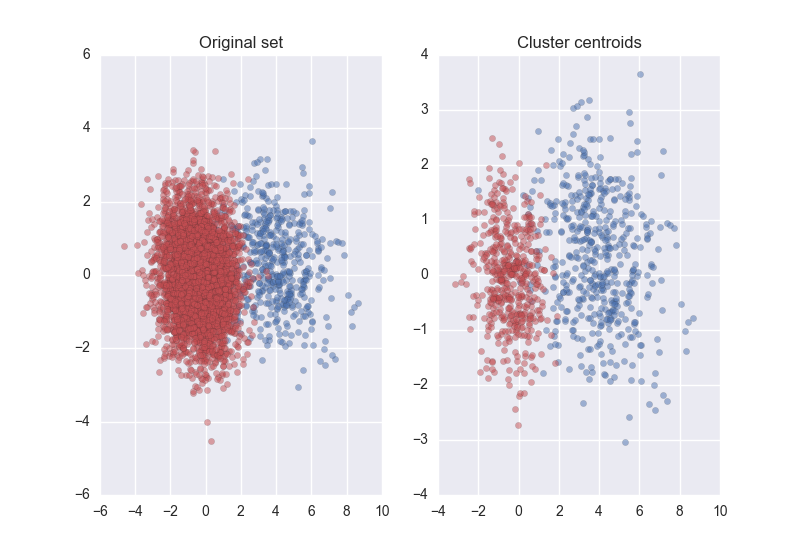
\includegraphics[width=0.3\linewidth]{sphx_glr_plot_cluster_centroids_001.png}} \hfill
%   \subfigure[]{\label{subfig:condensednearestneighbour}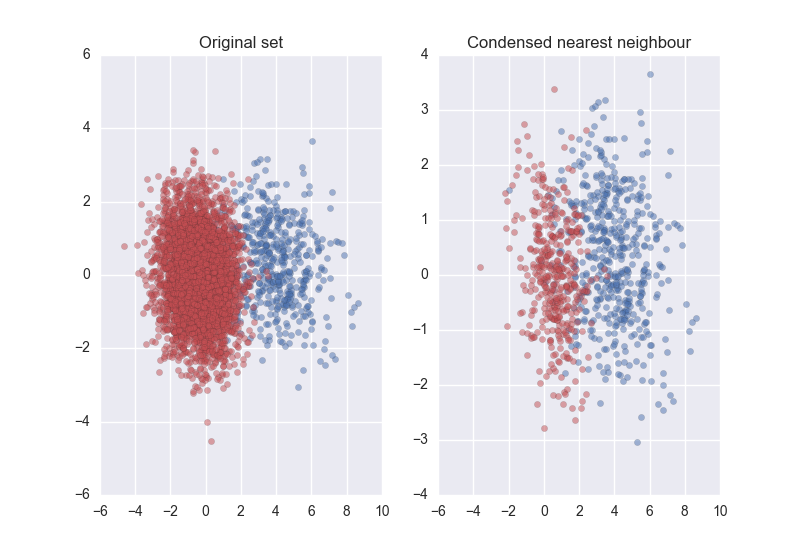
\includegraphics[width=0.3\linewidth]{sphx_glr_plot_condensed_nearest_neighbour_001.png}} \hfill
%   \subfigure[]{\label{subfig:editedneasrestneighbours}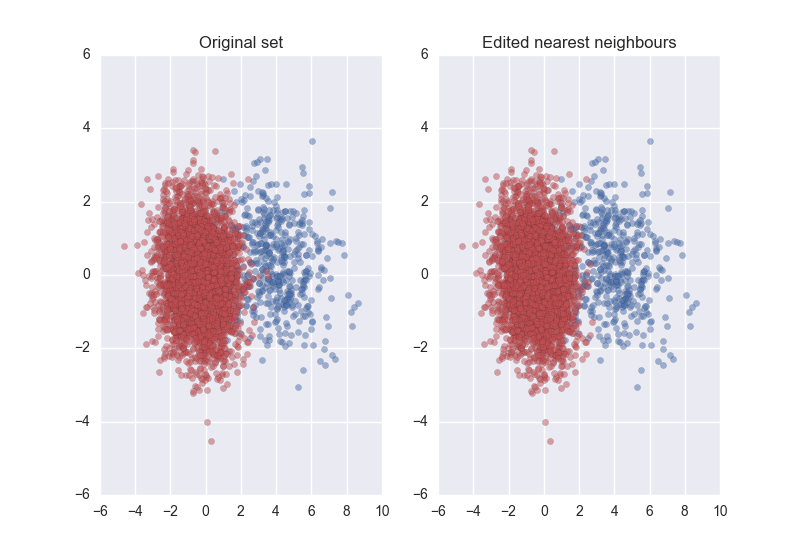
\includegraphics[width=0.3\linewidth]{sphx_glr_plot_edited_nearest_neighbours_001.png}}
%   \hspace*{\fill}\\
%   \hspace*{\fill}
%   \subfigure[]{\label{subfig:nearmiss1}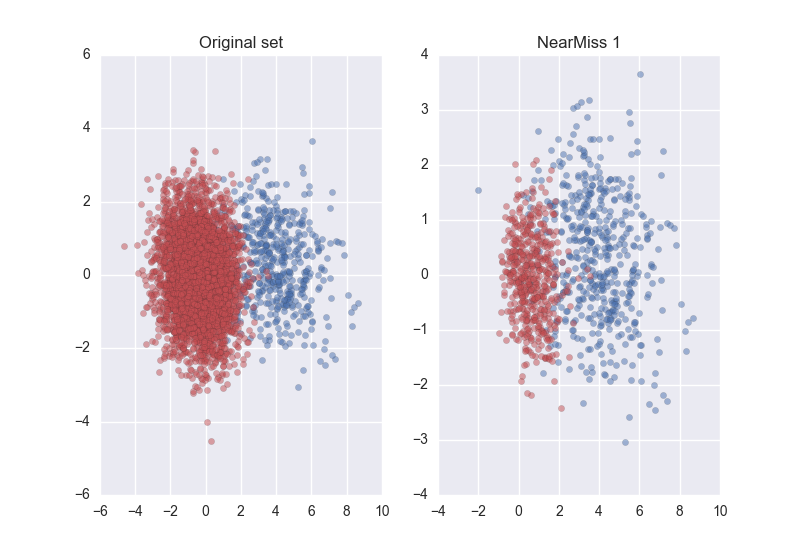
\includegraphics[width=0.3\linewidth]{sphx_glr_plot_nearmiss_1_001.png}} \hfill
%   \subfigure[]{\label{subfig:nearmiss2}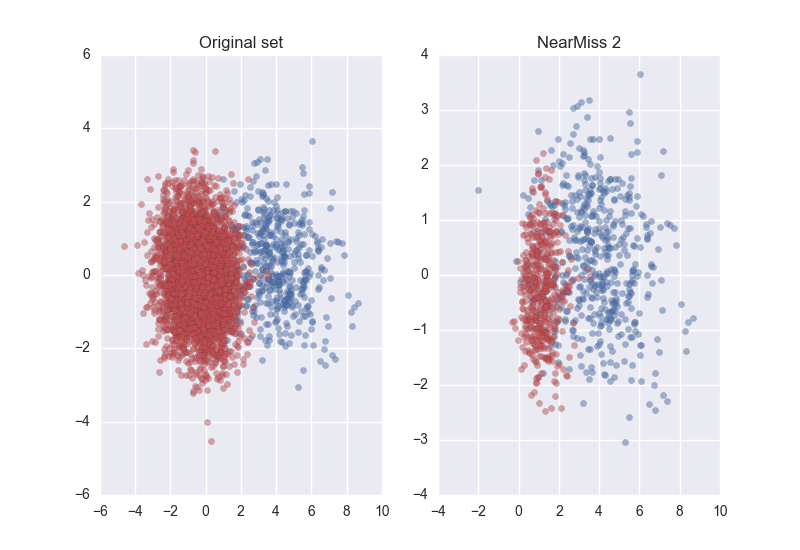
\includegraphics[width=0.3\linewidth]{sphx_glr_plot_nearmiss_2_001.png}} \hfill
%   \subfigure[]{\label{subfig:nearmiss3}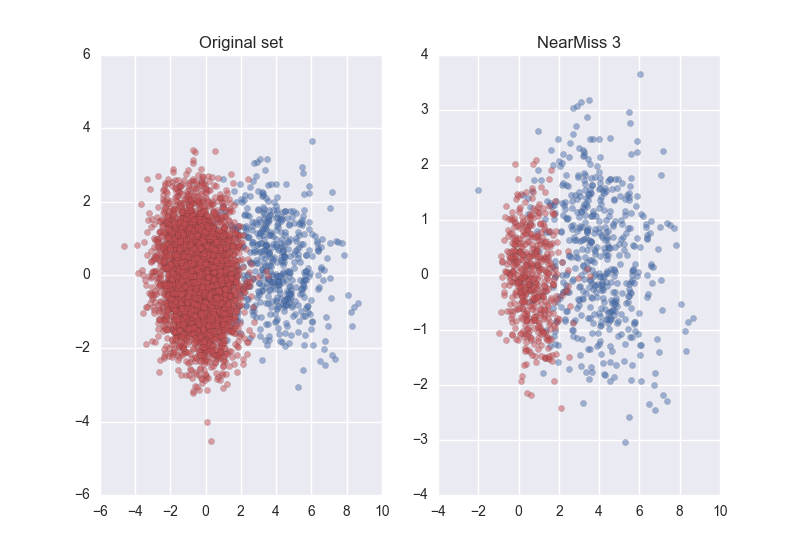
\includegraphics[width=0.3\linewidth]{sphx_glr_plot_nearmiss_3_001.png}}
%   \hspace*{\fill}\\
%   \hspace*{\fill}
%   \subfigure[]{\label{subfig:onesidedselection}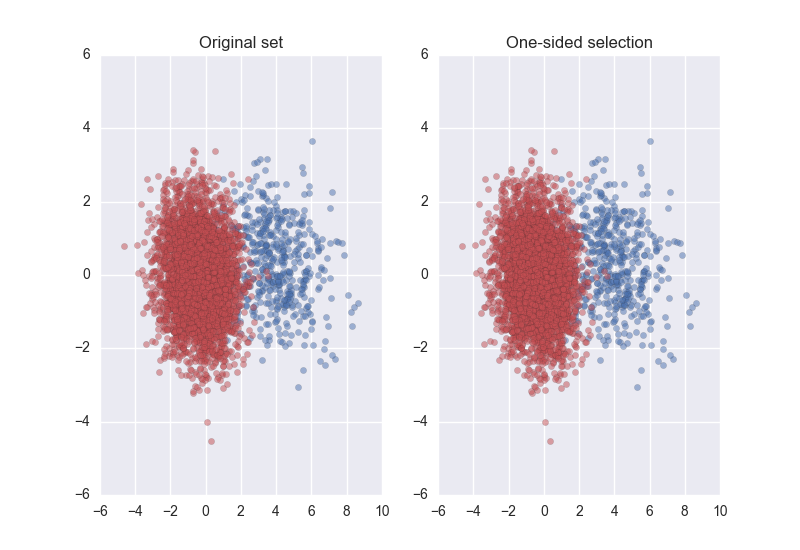
\includegraphics[width=0.3\linewidth]{sphx_glr_plot_one_sided_selection_001.png}} \hfill
%   \subfigure[]{\label{subfig:neighbourhoodcleaningrule}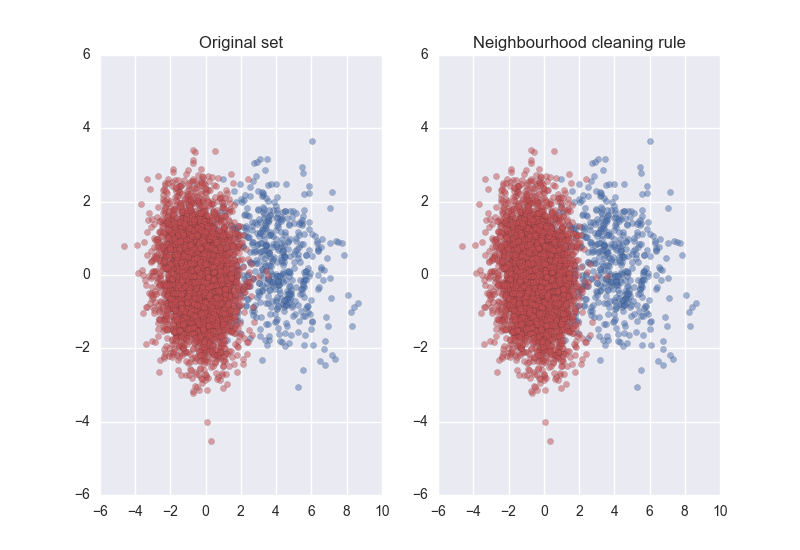
\includegraphics[width=0.3\linewidth]{sphx_glr_plot_neighbourhood_cleaning_rule_001.png}} \hfill
%   \subfigure[]{\label{subfig:tomeklinks}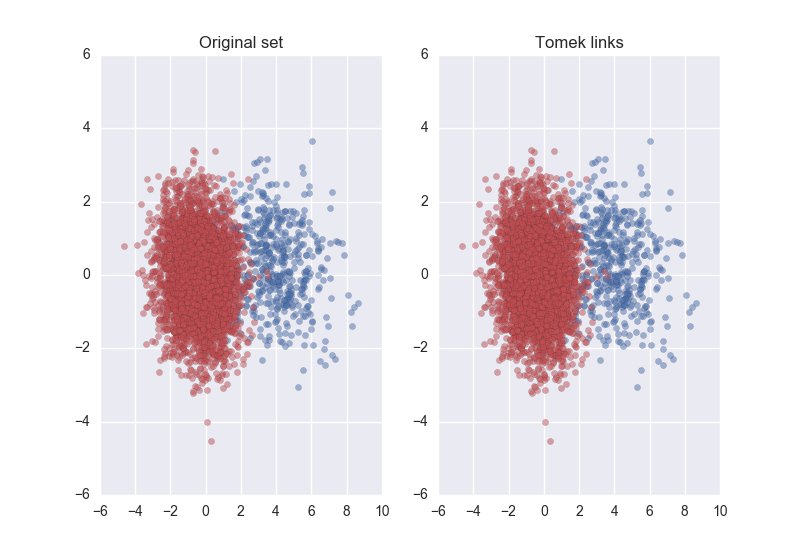
\includegraphics[width=0.3\linewidth]{sphx_glr_plot_tomek_links_001.png}}
%   \hspace*{\fill}\\
%   \hspace*{\fill}
%   \subfigure[]{\label{subfig:smote}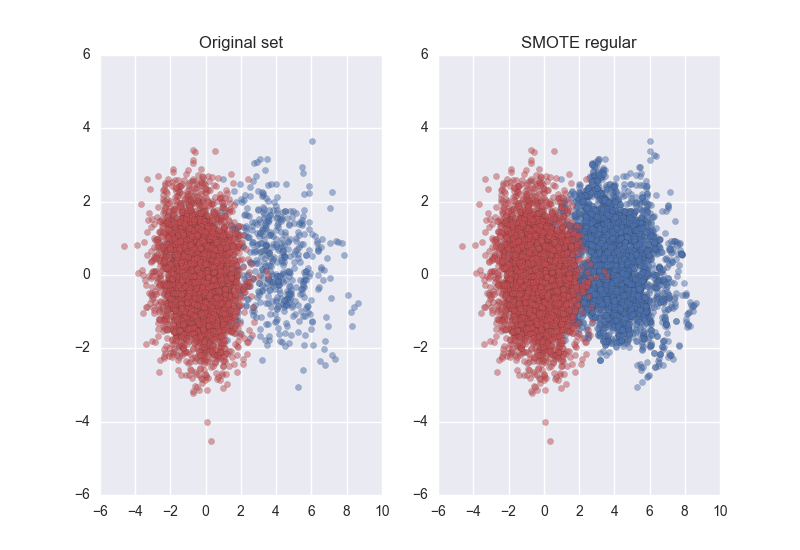
\includegraphics[width=0.3\linewidth]{sphx_glr_plot_smote_001.png}} \hfill
%   \subfigure[]{\label{subfig:smoteborderline1}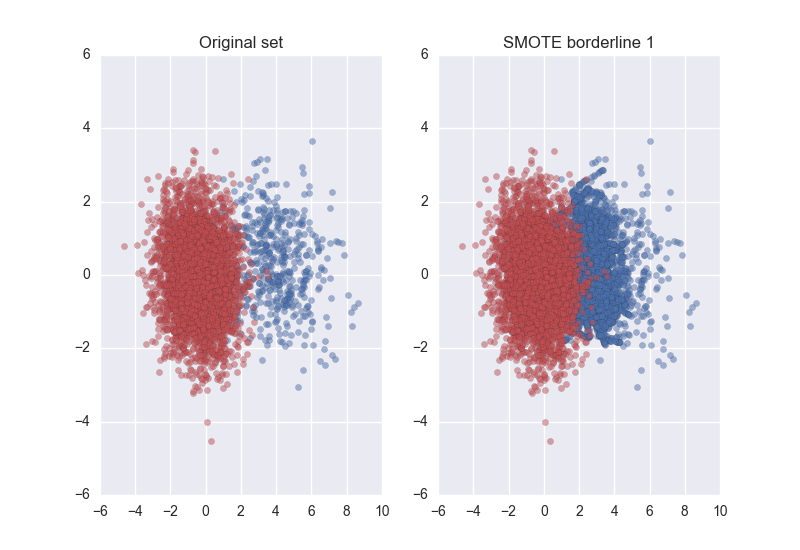
\includegraphics[width=0.3\linewidth]{sphx_glr_plot_smote_bordeline_1_001.png}} \hfill
%   \subfigure[]{\label{subfig:smoteborderline2}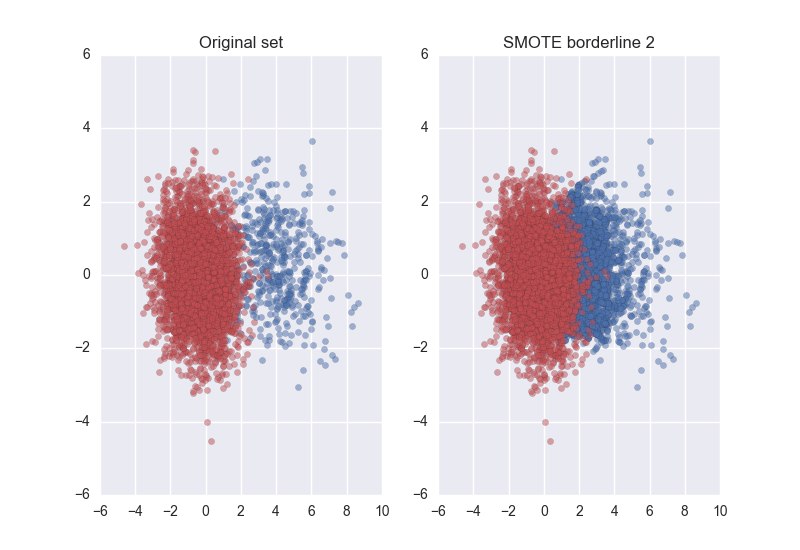
\includegraphics[width=0.3\linewidth]{sphx_glr_plot_smote_bordeline_2_001.png}}
%   \hspace*{\fill}\\
%   \hspace*{\fill}
%   \subfigure[]{\label{subfig:smotesvm}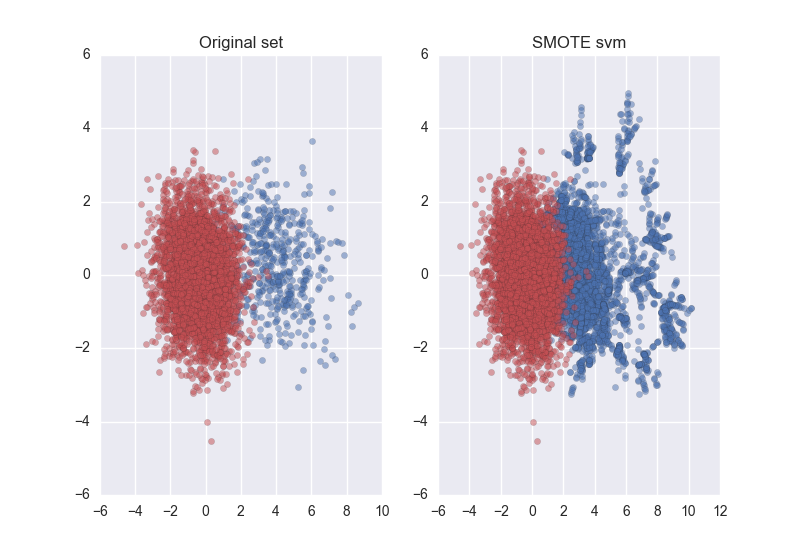
\includegraphics[width=0.3\linewidth]{sphx_glr_plot_smote_svm_001.png}} \hfill
%   \subfigure[]{\label{subfig:smoteenn}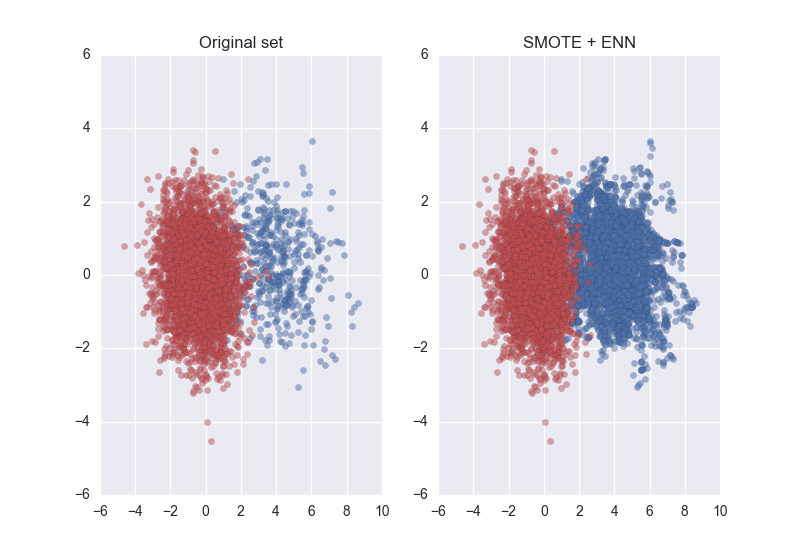
\includegraphics[width=0.3\linewidth]{sphx_glr_plot_smote_enn_001.png}} \hfill
%   \subfigure[]{\label{subfig:smotetomek}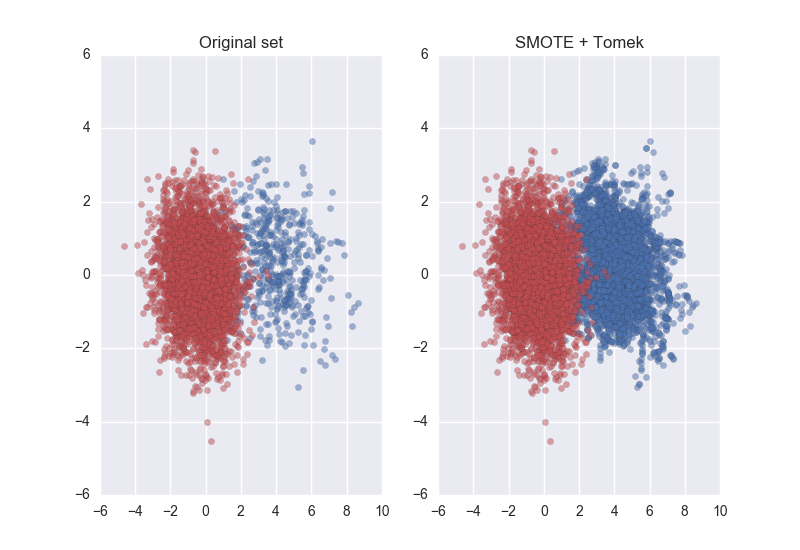
\includegraphics[width=0.3\linewidth]{sphx_glr_plot_smote_tomek_001.png}}
%   \hspace*{\fill}
%   \caption{Toy examples for the different sampling methods.}
%   \label{fig:methods}
% \end{figure}

\section{Conclusion}

\acks{We would like to acknowledge support for this project
from GitHub, Travis CI, and Gitter.}

\bibliography{bibtex}


\end{document}
